\documentclass[12pt]{report}

% includes
\usepackage{geometry}           % page size
\usepackage[utf8]{inputenc}     % encoding
\usepackage{palatino}           % font
% \usepackage[romanian]{babel}    % language
\usepackage[english]{babel}
\usepackage{graphicx}           % images
\usepackage{indentfirst}        % indentation
\usepackage[nottoc]{tocbibind}  % table of contents style
\usepackage[unicode]{hyperref}  % references from the table of contents
\usepackage{amsmath}
\usepackage[
    n,
    operators,
    advantage,
    sets,
    adversary,
    landau,
    probability,
    notions,    
    logic,
    ff,
    mm,
    primitives,
    events,
    complexity,
    asymptotics,
    keys]{cryptocode}
\usepackage{float}
\usepackage{xcolor}
\usepackage{changepage}
\usepackage{algorithm}
\usepackage{algpseudocode}
\usepackage{tikz}
\usetikzlibrary{arrows.meta, positioning}
\usepackage{caption}
\usepackage{mathtools}
\usepackage{amssymb}

% includes options
\geometry{  a4paper,            % scientific thesis standard
            left=2.5cm,
            right=2.5cm,
            top=2cm,
            bottom=2cm,
 }
\graphicspath{{images/}}        % path where the images are located
\setlength{\parindent}{1cm}     % paragraph indentation

% other options
\linespread{1.5}                % space between lines
\renewcommand*\contentsname{Contents}    % table of contents name

% the document content
\begin{document}
    % macros (global)
    \newcommand{\university}    {"Alexandru-Ioan Cuza" University Iași}
\newcommand{\universityg}   {of "Alexandru-Ioan Cuza" University Iași} % genitive
\newcommand{\faculty}       {Faculty of Computer Science}
\newcommand{\facultyg}      {of Faculty of Computer Science} % genitive
\newcommand{\speciality}    {Computer Science}
\newcommand{\promotion}     {2025}                                  %<---------

\newcommand{\thesistype}    {Bachelor's thesis}
\newcommand{\thesistitle}   {Consequences of using temporary variables in RFID authentication}    %<---------

\newcommand{\authorlast}    {Patrașcan}                               %<---------
\newcommand{\authorfirst}   {Andrei-Alexandru}
\newcommand{\authornamefl}  {\authorfirst \space \authorlast} % first name first
\newcommand{\authornamelf}  {\authorlast \space \authorfirst} % last name first
\newcommand{\authorbirth}   {22 martie 1999}                      %<---------
\newcommand{\authoraddress} {România, jud. Bacău, com. Filipești, sat Hârlești, str. Zorilor, nr. 180} %<---------
\newcommand{\authorcnp}     {1990322046190}                         %<---------

\newcommand{\session}       {july, 2025}                       %<---------
\newcommand{\coordinator}   {Prof. Dr. Țiplea Ferucio Laurențiu}               %<---------

\newcommand{\dottedline}    {............................}
    
    % front-matter
    \pagenumbering{gobble}
    
    % define the cover page
\begin{titlepage}
    \begin{center}
        % the university and faculty
        \large
        \MakeUppercase{\university}
        
        \LARGE
        \textbf{\MakeUppercase{\faculty}}
        
        % the faculty logo
        \vspace{1cm}
        
\includegraphics[width=0.3\textwidth]{logoFii.png}
        
        % thesis title
        \vspace{1cm}
        \Large
        \MakeUppercase{\thesistype}
        
        \vspace{0.5cm}
        \LARGE
        \textbf{\thesistitle}
        
        % author
        \vspace{2cm}
        \Large
        propusă de
        
        \vspace{0.5cm}
        \LARGE
        \textbf{\authornamefl}
        
        % session
        \vfill
        \Large
        \textbf{Sesiunea:} \session
        
        % scientific coordinator
        \vspace{2cm}
        \Large
        Coordonator științific
        
        \vspace{0.5cm}
        \LARGE
        \textbf{\coordinator}
    \end{center}
\end{titlepage}
    % define the title page
\begin{titlepage}
    \begin{center}
        % the university and faculty
        \large
        \MakeUppercase{\university}
        
        \LARGE
        \textbf{\MakeUppercase{\faculty}}
        
        % thesis title
        \vspace{8cm}
        \huge
        \textbf{\thesistitle}
        
        % author
        \vspace{2cm}
        \LARGE
        \textbf{\authornamefl}
        
        % session
        \vfill
        \Large
        \textbf{Sesiunea:} \session
        
        % scientific coordinator
        \vspace{4cm}
        \Large
        Coordonator științific
        
        \vspace{0.5cm}
        \LARGE
        \textbf{\coordinator}
    \end{center}
\end{titlepage}
    \vspace*{\fill}

\begin{flushright}
    Avizat, \\
    Îndrumător lucrare de licență, \\
    \coordinator. \\
    Data: \dottedline \hspace{1cm} Semnătura: \dottedline
\end{flushright}

\vspace{1cm}
\begin{center}
    \large
    \textbf{Declarație privind originalitatea conținutului lucrării de licență}
\end{center}

Subsemnatul \textbf{\authornamelf} domiciliat în \textbf{\authoraddress}, născut la data de \textbf{\authorbirth}, identificat prin 
CNP \textbf{\authorcnp}, absolvent al \facultyg, \textbf{\faculty} specializarea \textbf{\speciality}, promoția \promotion, declar 
pe propria răspundere cunoscând consecințele falsului în declarații în sensul art. 326 din Noul Cod Penal și dispozițiile Legii Educației 
Naționale nr. 1/2011 art. 143 al. 4 și 5 referitoare la plagiat, că lucrarea de licență cu titlul \textbf{\thesistitle} elaborată sub 
îndrumarea domnului \textbf{\coordinator}, pe care urmează să o susțin în fața comisiei este originală, îmi aparține și îmi asum 
conținutul său în întregime.

De asemenea, declar că sunt de acord ca lucrarea mea de licență să fie verificată prin orice modalitate legală pentru confirmarea 
originalității, consimțind inclusiv la introducerea conținutului ei într-o bază de date în acest scop.

Am luat la cunoștință despre faptul că este interzisă comercializarea de lucrări științifice în vederea facilitării falsificării de 
către cumpărător a calității de autor al unei lucrări de licență, de diplomă sau de disertație și în acest sens, declar pe proprie 
răspundere că lucrarea de față nu a fost copiată ci reprezintă rodul cercetării pe care am întreprins-o.

\begin{flushright}
    Data: \dottedline \hspace{6cm} Semnătura: \dottedline
\end{flushright}

\vspace*{\fill}
\pagebreak
    \vspace*{\fill}
\begin{center}
    \large
    \textbf{Declarație de consimțământ}
\end{center}

Prin prezenta declar că sunt de acord ca lucrarea de licență cu titlul \textbf{\thesistitle}, codul sursă al programelor și celelalte 
conținuturi (grafice, multimedia, date de test, etc.) care însoțesc această lucrare să fie utilizate în cadrul Facultății de informatică.

De asemenea, sunt de acord ca Facultatea de informatică de la Universitatea ”Alexandru-Ioan Cuza” din Iași, să utilizeze, modifice, 
reproducă și să distribuie în scopuri necomerciale programele-calculator, format executabil și sursă, realizate de mine în cadrul 
prezentei lucrări de licență.

\begin{flushright}
    Absolvent \textbf{\authornamefl} \\
    \vspace{0.5cm}
    Data: \dottedline \hspace{6cm} Semnătura: \dottedline
\end{flushright}
\vspace*{\fill}
\pagebreak
    
    % table of contents
    \tableofcontents
    
    % chapters
    \setcounter{page}{1}
    \pagenumbering{arabic}
    
    \chapter*{Motivation} 
\addcontentsline{toc}{chapter}{Motivation}

The choice towards studying RFID schemes and their security came for multiple reasons. 

Firstly the applications for this fascinating technology are vast, they provide near-instant authentication for multiple tags 
at the same time meaning it can be used in the medical field, for supply chains, in the automotive and construction industry and where 
it all started, in a military context. They provide access control from authentication of staff to providing access to ski lifts.

Secondly a typical RFID scheme is an environment where achieving security properties is difficult. The tags come with multiple 
constraints like processing power and limited memory and some of them can only work when interacting with a reader. This means 
that the RFID protocols need to strike a balance between lightness of operations and a solid security parameter. 
The tags are also cheap devices that are not tamper-proof, meaning new difficulties in developing solid protocols concerning how
memory is used.

All these limitations and the possible applications of RFID schemes lead to a challenging but rewarding 
field of study.
    \chapter*{Introduction} 
\addcontentsline{toc}{chapter}{Introduction}

    In a world that grows more and more a reliability on smart devices the need for secure and private protocols grows with it. One 
such technology that makes this possible is RFID. RFID is the acronym of \textbf{Radio Frequency Identification} and it designates
a wireless technology that uses radio signals aiming to identify objects and persons by the means of devices (tags) attached to them.

    During World-War II, the British wanted to distinguish between enemy and their own returning aircraft. To achieve this they placed transponders
on their aircraft which would respond to queries from the base stations. This was called the Identity Friend or Foe (IFF) system, which is considered to be the
first use of RFID.

    Since then RFID technology has been applied to a number of technical and scientific fields. In medicine RFID tags are used in blood transfusion and analysis. 
A RFID reader scans the tags attached to blood bags and finds the appropriate one for a specific patient. In the aeronautics industry, 
RFID tags are used for the supply chain. In the automotive industry, the tags can be attached to parts of a car and tracked during assembly.
RFID also has many applications in the construction industry \cite{Domdouzis}, from automated tracking of pipe spools to tracking the 
location of buried assets.
    \section*{Use of AI} 
\addcontentsline{toc}{section}{Use of AI}

The short following section covers the use of artificial intelligence. AI has had major impact on the educational process and a section 
presenting the use of this tool contributes to the work's academic integrity.

The development of this work included the use of AI in one regard, that of strictly consulting on the available works relevant to
the subject at hand. This has been done for the purpose of achieving a holistic view of the subject. 
    \chapter{Security and Privacy in Vaudenay's RFID model}

\section{RFID Schemes}

        A typical RFID system includes three components: a coil (or antenna), a transceiver (with a decoder) and a
    transponder(a radio-frequency tag) embedded with unique information. The antenna emits radio signals in order to activate the tag and 
    to read or write data on it. Antennas establish the communication between the transceiver and the tags. They can be packaged with 
    the transceiver and the decoder in order to become a reader. 

        \textbf{The tags} are passive transponders identified by a unique ID. Their technical parameters often are: memory, power supply, shape, size and the presence of a 
    microprocessor. For many applications the tags need to be very small and cheap so their attributes are deeply constrained. A tag most often:
    \begin{itemize}
        \item is passive: because it has no batteries it can operate only when queried by the reader and can only respond for a short time after;
        \item has limited memory: a few kilobits of memory;
        \item has limited computational ability, can only perform basic calculations: hash calculations \cite{Feldhofer}, pseudorandom generation \cite{Robshaw}, 
        symmetric encryption \cite{Feldhofer2}. Some elliptic-curve arithmetic and public-key cryptography may fit, but remain expensive so far;
        \item provides no physical security: each tag can be opened(corrupted) and thus revealing its memory;
        \item communicates at up to a fixed distance: the tag has a range of a few meters.
    \end{itemize}
    
    In RFID Moore's law cannot be directly applied. In fact, the main goal of RFID transponders producers is to keep prices down and so the performance takes
    a secondary, less important role.

        \textbf{The reader} is composed by one or more transceivers and a backend processing system(sometimes in the literature the reader denotes just the transceiver). 
    The reader is able to accomodate multiple tags at the same time although a high number of them can lead to substantial delays for authentication. 
    
        \textbf{The server} is the component that handles the complex cryptographic calculations and eases the load on readers whenever possible. The traditional protocols
    included fixed reader positions and assumed secure(wired) communication. However in practical applications the communication between server and reader is also done via 
    Radio-Frequency Signals.

        RFID protocols are used most often for two goals: to identify tags(by recovering their unique ID) and to authenticate tags(to make sure a tag is legitimate i.e. registered in 
    the database). 

        A frequently used and accepted model for security and privacy for RFID schemes is Vaudenay's
    model, proposed in \cite{Vaudenay}. 

    \textbf{RFID schemes}: A RFID scheme is formed by a triple:

    - a setup scheme for the reader: SetupReader($\lambda$): generates a pair of keys: $K_P$ and 
    $K_S$ for the reader depending on the security parameter $\lambda$. The public key is released
    to the public and the secret key is stored on the reader database.

    -a setup scheme for the tag: SetupTag(ID) $\rightarrow$ (K, S): K is the tag secret and S denotes the 
    initial state of the tag. Furthermore if the tag is legitimate the values ID and K are stored
    on the memory of the reader.
    
    -an interactive protocol between the reader and the tag, at the end of comunication the reader
    will output a value ($\bot$, correct ID, incorrect ID) indicating succesfull authentication or 
    not and the tag returns $ok$ for a legitimate reader or $\bot$ otherwise. Formally:
    $Ident[\mathcal{T}_{ID}:S; \mathcal{R}: sk_{\mathcal{R}}, DB; *:pk_{\mathcal{R}}] \rightarrow 
    [\mathcal{T}_{ID}:out_{\mathcal{T}_{ID}}; \mathcal{R}:out_{\mathcal{R}}]$. This is interpreted as:
    the identification protocol "Ident" starts with tag $\mathcal{T}_{ID}$ from state $S$, the reader $R$ having the secret key 
    $sk_{\mathcal{R}}$ and the access to database $DB$, and public key $pk_{\mathcal{R}}$ being shared to both parties. After a 
    succesfull computation it leads to $\mathcal{T}_{ID}$ returning $out_{\mathcal{T}_{ID}}$ and $\mathcal{R}$ yielding $out_{\mathcal{R}}$.

    The \textit{correctness} of a RFID scheme means that after each succesfull execution of the interactive protocol between the reader and a 
    legitimate tag, the reader outputs the tag's identify with overwhelming probability. For mutual authentication schemes correctness also includes
    that the tag outputs $ok$ with overwhelming probability.

\section{Adversaries and oracles}

    \textit{Adversaries:} An adversary is often defined by what action they can perform, i.e. the oracles they can query, 
    the goals of their attack(also known as the game they are playing) and by the way they can interact with a system. An adversary
    is a PPT algorithm.
    
    A tag can be either \textit{drawn} or \textit{free}, this means that it is in reach or not of the 
    adversary. A virtual tag is a temporary identifier for a tag when it is drawn.

    Below are the 8 oracles defined in Vaudenay's model:

    1. \textit{$CreateTag^b$(ID)}: created a new tag, legitimate(b=1) or illegitimate(b=0) with the unique ID.
        This oracles uses SetupTag(ID) and if the tag is legitimate then the reader 
        updates its database. The reader searches the database in order to authenticate tags.
    
    2. \textit{DrawTag($distr) \rightarrow (vtag_1, b_1, ... , vtag_n, b_n$)}: selects at random n tags following the 
    distribution $distr$ and draws them to be used by the adversary. The oracle provides
    an array of virtual identifiers ($vtag_1, ... ,vtag_n$) as the adversary needs to reference them.
    and the bits $b_k$ meaning authentic or not. 
    
    A hidden table $\Gamma$ is kept by the oracle containing the association between the temporary identifiers and the real IDs.
    This will be revealed after an attack experiment to determine if it was succesfull or not.

    3. \textit{Free(vtag)}: the vtag is eliminated from the set the attacker works with. This makes it unreachable to the adversary.
    
    4. \textit{Launch $\rightarrow \pi$}: the reader launches a new protocol instance $\pi$.

    5. \textit{SendReader($m, \pi) \rightarrow (m'$)}: sends the reader a message m and receives as response 
    the message $m'$ as part of the protocol $\pi$.

    6. \textit{SendTag($m, \pi) \rightarrow (m'$)}: sends the tag a message m and receives as response 
    the message $m'$. If m is empty the response is the first message transmitted by the tag for
    a given protocol. 

    7. \textit{Result($\pi$)}: After the protocol has ended on the reader side, output 1 if the tag was 
    authenticated and 0 otherwise.

    8. \textit{Corrupt(vtag)}: Outputs the current internal state of the tag temporary named vtag. 

    \section{Classes of adversaries}
    Depending on how these oracles are used/the access the attacker has, 4 kinds of adversary are defined:
    
    1. \textit{STRONG}: class of adversary who have access to all the oracles, no limitations on how the Corrupt(vtag) oracle
    is used. Thus a strong adversary can get the state of a tag and still query other oracles for tag $\mathcal{T}$.

    2. \textit{DESTRUCTIVE}: adversaries who never use a tag after a Corrupt(vtag) oracle is called
        i.e. the tag is destroyed.

    3. \textit{FORWARD}: adversaries that once they call Corrupt(vtag) oracles can only call the same oracle
        i.e the corruption of tags are left at the end of the attacking phase.

    4. \textit{WEAK}: adversaries who have no access to the Corrupt(vtag) oracle, the internal memory of the tags remains a secret. 

    Another way to consider adversaries is by their access to the Result($\pi$) oracle. If they have the access, they are considered to be
    \textit{wide} adversaries, if not, they are called \textit{narrow}. Since the access to the Corrupt() and the Result() oracles
    is quite orthogonal 4 new distinct adversarial models are distinguished: narrow-strong, narrow-destructive, narrow-forward and narrow-weak.

\section{Security}

    The security definition of the Paise-Vaudenay model \cite{PV model} encompases attacks where the adversary aims to impersonate or 
    forge a legitimate tag $\mathcal{T}$ or the reader $\mathcal{R}$.

    Consider an adversary in the class STRONG. They win if there is an instance of the protocol run
    by the reader where a legitimate tag is authenticated but done so when the specific steps of the 
    protocol are followed out of order(interleaved). If the probability of the adversary to win is 
    negligible then a RFID scheme is considered secure.

    For a mutual authentication scheme the same property also needs to be respected for the tag authenticating
    the reader.

    \textit{Reader authentication}: The definition of reader authentication is based on a security experiment $Exp_{\mathcal{A}_{sec}}^{\mathcal{R}-aut}$
    where a strong adversary must impersonate $\mathcal{R}$ to a legitimate tag $\mathcal{T}_{ID}$. To exclude trivial attacks, the attacker $\mathcal{A}_{sec}$
    must compute some of the protocol messages, not just forward them from $\mathcal{R}$ to $\mathcal{T}_{ID}$. $Exp_{\mathcal{A}_{sec}}^{\mathcal{R}-aut}$ = 1
    denotes that $\mathcal{A}_{sec}$ wins the security experiment.

    \textbf{Definition 1}: An RFID system achieves reader authentication if for every strong adversary $\mathcal{A}_{sec}$, probability 
    Pr[$Exp_{\mathcal{A}_{sec}}^{\mathcal{R}-aut}$ = 1] is negligible.

    \section{Privacy}

    Vaudenay's notion of privacy captures anonymity and unlinkability and focuses on the privacy loss in the wireless link. It is based on 
    the existence of a simulator $\mathcal{B}$, called a \textbf{blinder}, that can simulate the reader and the tags without knowing their secrets.
    
    The simulation aspect of the blinder catches the case of an adversary that can't use the messages transmitted, they only know how the protocol
    interacts and the actual data traffic is simulated. By contrasting this attacker with an adversary that eavesdropes, denies or changes messages
    several conclusions can be drawn about the leakage of data and the privacy of a protocol.

    The privacy definition can be formalized by a privacy experiment $Exp_{\mathcal{A}_{prv}}^{prv-b} = b^{'}$ defined by an adversary of class P, a
    security parameter s and $b \in_{R} \{0,1\}$. In the first phase of the experiment, the reader is initialized (using SetupReader($1^s$)). 
    The public key is available to $\mathcal{A}_{prv}$ and $\mathcal{B}$. $\mathcal{A}_{prv}$ interacts with the protocol according to its constraints.
    If b = 1, all queries to Launch, SendReader, SendTag and Result oracles are handled by $\mathcal{B}$. Moreover, the blinder can surveil all the other
    oracles. In phase two, the adversary cannot call the oracles any longer but is given the hidden table $\Gamma$ of the DrawTag oracle. Finally, 
    $\mathcal{A}_{prv}$ returns bit $b^{'}$.

    Informally, $Pr[Exp_{\mathcal{A}_{prv}}^{prv-b}]$ denotes the probability that an adversary $\mathcal{A}_{prv}$
    can guess the bit b, meaning whether they interact with the real oracles or through a blinder $\mathcal{B}$.

    \textbf{Definition 2}: Let P be one of the adversary classes specified above. An RFID system is P-private if for
    every adversary $\mathcal{A}_{prv}$ of P there exists a probabilistic polynomial time algorithm $\mathcal{B}$ 
    (blinder) such that the advantage $Adv_{\mathcal{A}_{prv}}^{prv} = | Pr[Exp_{\mathcal{A}_{prv}}^{prv-0} = 1] - Pr[Exp_{\mathcal{A}_{prv}}^{prv-1} = 1] |$ 
    of $\mathcal{A}_{prv}$ is negligible. $\mathcal{B}$ simulates the oracles: Launch, SendReader, SendTag and
    Result to $\mathcal{A}_{prv}$ without having access to the reader's secret key or database. It is considered the all
    oracle queries $\mathcal{A}_{prv}$ makes and the responses received are also available to $\mathcal{B}$.

    Privacy is defined by the ability of the adversary to infer relations about the ID from the protocol
    messages. If a scheme is resistent to all P-private adversaries(belonging to P class, with all
    P specific access) then the scheme achieves P-privacy.

    An adversary $\mathcal{A}$ is \textit{trivial} if there is a negligible difference between the chances
    of an adversary that interacts with the system to win and the chances of a blinded adversary.

    All privacy notions defined in the Paise-Vaudenay Model are linked the following way:

    \[
    \begin{array}{|ccccccc|}
        \hline
        \text{Strong} & \Rightarrow & \text{Destructive} & \Rightarrow & \text{Forward} & \Rightarrow & \text{Weak} \\
        \Downarrow & &  \Downarrow  & &\Downarrow  & & \Downarrow \\
        \text{Narrow-Strong} & \Rightarrow & \text{Narrow-Destructive} & \Rightarrow & \text{Narrow-Forward} & \Rightarrow & \text{Narrow-Weak} \\
        \hline
    \end{array}
    \]

    Remark: The following relation is clear: $Weak \subseteq Forward \subseteq Destructive \subseteq Strong$.

    This means that if a particular class of privacy is proven to be impossible for a given set of parameters then the protocol can achieve 
    a weaker class. For example if destructive privacy is unachievable then the protocol can still be narrow-destructive or forward private.

    \chapter{RFID Authentication}

\section{Primitives used}
    The chosen paper\cite{BOM}'s authentication is presented in the following chapter. The Protocol makes use of a diagonal block key matrix (DBKM) encryption algorithm for it's property of 
    expanding the key size of the encryption without need of extensive resources. It insurres a balance between security and lightness of operations. Another component is the self updating encryption 
    order (SUEO) and it's role is to boost security. Lastly a self updating modulus (SUM) algorithm is deployed to weaken the correlation between the plaintext and the ciphertext.
    
    These three algorithms are used to form the block-order-modulus variable matrix encryption algorithm, dubbed the DBKM-SUEO-SUM algorithm.

\section{Primitives' structure}

    \cite{BOM} proposes 3 corollaries based on block matrix properties and modulo operations that make the base for the primitives.

    A. \textbf{DBKM}

    For two square matrices $A_1$ and $A_2$: if $A_1 \times t_1$ mod(p) = $c_1$ and $A_2 \times t_2$ mod(p) = $c_2$ exist then:
    \begin{gather*}
        \begin{pmatrix}
        A_1 &  \\
            & A_2
        \end{pmatrix}
        \times
        \begin{pmatrix}
            t_1  \\
            t_2
        \end{pmatrix}
        mod(p)
        =
        \begin{pmatrix}
            c_1  \\
            c_2
        \end{pmatrix}
    \end{gather*}

    Updating the order of the first matrix along the main diagonal yields multiple key matrices of different sizes thus expanding the key size. For the fact that 
    it uses 2 matrices $A_1$ and $A_2$ as its building blocks the tag does not need to keep multiple separate keys in its memory.

    B. \textbf{SUEO}

    For 2 square matrices $A_1$ and $A_2$: if $A_1 \times t$ mod(p) = $c_1$ and $A_2 \times c_1$ mod(p) = $c_2$ exist and $A_2 \times t$ mod(p) = $c_3$ and 
    $A_1 \times c_3$ mod(p) = $c_4$ exist then: 
    
    \begin{gather*}
        c_2 \neq c_4
    \end{gather*}

    Using the property of non-commutativity of matrices one can change the order of the multiplications to get different ciphertexts. This change is equivalent to having multiple keys for
    encryption but with this result security can be improved without using additional storage space.

    C. \textbf{SUM}

    For 2 square matrices $A$ and $B$ and $A \times B$ = $I$(identity matrix)mod(p) then: 
    
    \begin{gather*}
        \textit{B is the modulus p-inverse matrix of A and the modulus q-inverse of A,}\\
        \textit{for a q integer divisor of p.}
    \end{gather*}

    Thus the change in modulus still yields an inverse and the decryption process can still happen but the correlation between the ciphertext and the plaintext is weakened.

    D. \textbf{DBKM-SUEO-SUM}

    The above three components can be used for an encryption and decryption algorithm. The following figure represents an example with two key matrices and three
    integer divisors of modulus p.

    \begin{center}
    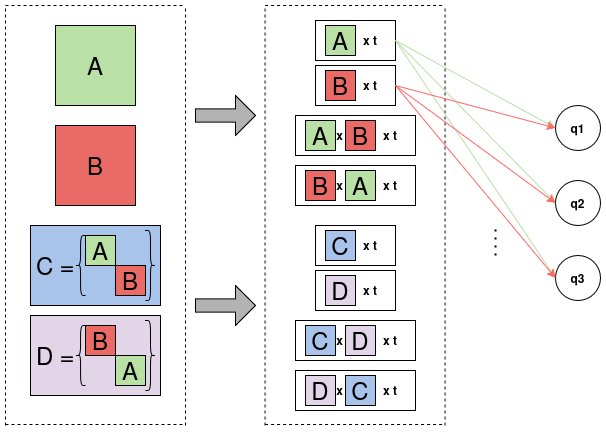
\includegraphics[width=0.7\textwidth]{Protocol_base_scheme.png}
    \end{center}

\section{Specific steps of the authentication protocol}

\begin{table}[H]
    \centering
    \caption{Notation used in the description of the protocol}
    \begin{tabular}{| c | c |}
        \hline
        Notation & Meaning \\
        \hline
        $N_t$ & Nonce generated by the tag \\
        $N_r$ & Nonce generated by the reader \\
        $S$ & Secret value \\
        $S_d$ & Secret value that determines the construction of the block key matrix  \\
        $S_p$ & Secret value that determines the encryption order  \\
        $S_c$ & Secret value that determines the selection of modulus  \\
        $p$ & Modulus  \\
        $q$ & q $\in$ f(p), f(p) is the set of integer divisors of p \\
        $Z$ &  Total number of DBKM index table \\
        $N$ &  Total number of key matrices \\
        $W_i$ & Total number of SUEO index table  \\
        $N_c$ & Total number of the set f(p)  \\
        $A, A_{new}$ & Initial and updated encryption matrices \\
        $B, B_{new}$ & Initial and updated decryption matrices \\
        \hline
    \end{tabular}
\end{table}

\noindent{
    The notation used in the protocol are shown in table 1. The details of it are are follows:

    1. The reader sends a query to the tag. This activates tags without batteries.

    2. The tag uses its internal pseudo-random number generator to get nonce $N_t$. After that the tag uses the encryption matrix A and the modulus p to encrypt $N_t||S$.

    3. The tag sends the message E($N_t||S$,A,p) to the reader. 

    4. The reader decrypts E($N_t||S$,A,p) and obtains the secret S. If S can be queried in its internal database, the reader has authenticated the tag succesfully and accepted nonce $N_t$, else the protocol is stopped. 
        After that, the reader generates nonce $N_r$ and uses A and p to encrypt $N_r||S$. 

    5. The reader sends E($N_r||S$,A,p) to the server. 

    6. The server decrypts E($N_r||S$,A,p) and obtains secret S. A query on S suggests a succesfull authentication of the reader in which case the server accepts $N_r$. Contrarily the protocol is stopped.
        The server generates the new secret values $S_d, S_p, S_c$ and uses A and p to encrypt $N_r||S_d||S_p||S_c$.

    7. The server sends E($N_r||S_d||S_p||S_c$,A,p) to the reader. 

    8. The reader decrypts E($N_r||S_d||S_p||S_c$,A,p) and obtains $N_r$. If the value $N_r$ received matches the saved value then the reader authenticates the server. In this case the new secret values 
        $S_d,S_p,S_c$ are accepted, if not the protocol is stopped. Afterwards the reader uses A and p to encrypt $N_t||S_d||S_p||S_c$. 

    9. The reader sends E($N_t||S_d||S_p||S_c$,A,p) to the tag. 

    10. The tag decrypts E($N_t||S_d||S_p||S_c$,A,p) and obtains $N_t$. If the value $N_t$ received matches the saved value then the tag authenticates the reader. Following that the new secret values 
        $S_d,S_p,S_c$ are accepted, if not the protocol is stopped. Subsequently fresh protocol parameters are calculted: mod($S_d$, Z) to determine the construction of diagonal block key matrix, 
        mod($S_p, W_i$) to determine the encryption order, mod($S_c, N_c$) to determine the choice of the new modulus. With the new key matrix $A_{new}$, new modulus q and encryption order, the tag 
        encrypts $N_t+1||ID$.

    11. The tag sends E($N_t+1||ID$,$A_{new}$,q) to the reader.
    
    12. Reader calculates mod($S_d$,Z), mod($S_p$,$W_i$), mod($S_c$,$N_c$) itself. Then it decrypts E($N_t+1||ID$,$A_{new}$,q) 
    using the newly calculted $B_{new}$ and q. If the value $N_t$ matches the saved value, ID is obtained. The reader uses $A_{new}$ and q to encrypt $N_r+1||ID$. 

    13. The reader sends E($N_r+1||ID$,$A_{new}$,q) to the server.

    14. Server calculates mod($S_d$,Z), mod($S_p$,$W_i$), mod($S_c$,$N_c$) itself. It decrypts E($N_r+1||ID$,$A_{new}$,q) using the newly calculted $B_{new}$ and q. If the value $N_r$ 
    matches the saved value, the server obtains ID.
    
}

% \newgeometry{left=1cm}

\begin{adjustwidth}{-60pt}{}
\procedureblock[colspace=-0.5cm]{The two way DBKM-SUEO-SUM-RFID authentication protocol}{
    \textbf{Server} \< \< \textbf{Reader} \< \< \textbf{Tag} \\[-1ex]
    \textit{A, B, p, f(p), S, Z, $W_i$} \< \< \textit{A, B, p, f(p),$N_r$, S, Z, $W_i$} \< \< \textit{A, B, p, f(p),$N_t$, S, Z, $W_i$} \\[-1.5ex]
    % \\
    \< \< \<\sendmessageright{top=\text{ \scriptsize 1.Query}} \< \\[-4ex]
    % \\
    \< \< \< \< \text{ \scriptsize 2.Generates $N_t$} \\[-1ex]
    \< \< \< \< \text{ \scriptsize E($N_t||S$,A,p)} \\[-4ex]
    % \\
    \< \< \< \sendmessageleft{top=\text{ \scriptsize 3.E($N_t||S$,A,p)}} \< \\[-4ex]
    % \\
    \< \< \text{ \scriptsize 4.D(E($N_t||S$,A,p),B,p)} \< \< \\[-1ex]
    \< \< \text{ \scriptsize Generates $N_r$} \< \< \\[-1ex]
    \< \< \text{ \scriptsize E($N_t||S$,A,p)} \< \< \\[-4ex]
    % \\
    \< \sendmessageleft{top=\text{ \scriptsize 5.E($N_r||S$,A,p)}} \< \< \< \\[-4ex]
    % \\
    \text{ \scriptsize 6.D(E($N_r||S$,A,p),B,p)} \< \< \< \< \\[-1ex]
    \text{ \scriptsize Generates $S_d, S_p, S_c$} \< \< \< \< \\[-1ex]
    \text{ \scriptsize E($N_r||S_d||S_p||S_c$,A,p)} \< \< \< \< \\[-4ex]
    % \\
    \< \sendmessageright{top = \text{ \scriptsize 7.E($N_r||S_d||S_p||S_c$,A,p)}} \< \< \< \\[-4ex]
    % \\
    \< \< \text{ \scriptsize 8.D(E($N_r||S_d||S_p||S_c$,A,p),B,p)} \< \< \\[-1ex]
    \< \< \text{ \scriptsize E($N_t||S_d||S_p||S_c$, A, p)} \< \< \\[-4ex]
    % \\
    \<\<\<\sendmessageright{top = \text{ \scriptsize 9.E($N_t||S_d||S_p||S_c$,A,p)}}\<\\[-4ex]
    % \\
    \< \< \< \< \text{ \scriptsize 10.D(E($N_t||S_d||S_p||S_c$,A,p),B,p)} \\[-1ex]
    \< \< \< \< \text{ \scriptsize Calculates mod($S_d$,Z)} \\[-1ex]
    \< \< \< \< \text{ \scriptsize Calculates mod($S_p$,$W_i$)} \\[-1ex]
    \< \< \< \< \text{ \scriptsize Calculates mod($S_c$,$N_c$)} \\[-1ex]
    \< \< \< \< \text{ \scriptsize E($N_t+1||ID$,$A_{new}$,q)} \\[-4ex]
    % \\
    \< \< \< \sendmessageleft{top=\text{ \scriptsize 11.E($N_t+1||ID$,$A_{new}$,q)}} \< \\[-4ex]
    % \\
    \< \< \text{ \scriptsize 12.Calculates mod($S_d$,Z)} \< \<\\[-1ex]
    \< \< \text{ \scriptsize Calculates mod($S_p$,$W_i$)} \< \<\\[-1ex]
    \< \< \text{ \scriptsize Calculates mod($S_c$,$N_c$)} \< \<\\[-1ex]
    \< \< \text{ \scriptsize D(E($N_t+1||ID$,$A_{new}$,q),$B_{new}$,q)} \< \<\\[-1ex]
    \< \< \text{ \scriptsize E($N_r+1||ID$,$A_{new}$,q)} \< \<\\[-4ex]
    % \\
    \< \sendmessageleft{top=\text{ \scriptsize 13.E($N_r+1||ID$,$A_{new}$,q)}} \< \< \< \\[-2ex]
    % \\
    \text{ \scriptsize 14.Calculates mod($S_d$,Z)} \< \< \< \<\\[-1ex]
    \text{ \scriptsize Calculates mod($S_p$,$W_i$)} \< \< \< \<\\[-1ex]
    \text{ \scriptsize Calculates mod($S_c$,$N_c$)} \< \< \< \<\\[-1ex]
    \text{ \scriptsize D(E($N_r+1||ID$,$A_{new}$,q),} \< \< \< \<\\[-1ex]
    \text{ \scriptsize $B_{new}$,q)} \< \< \< \<\\[-1ex]
    \text{ \scriptsize Obtains ID} \< \< \< \<\\[-4ex]
}
\end{adjustwidth}
    
% \restoregeometry
    \chapter{Third chapter title}

Amet venenatis urna cursus eget. Quam vulputate dignissim suspendisse in est ante. Proin nibh nisl condimentum id. Egestas maecenas 
pharetra convallis posuere morbi. Risus viverra adipiscing at in. Vulputate eu scelerisque felis imperdiet. Cras adipiscing enim eu 
turpis egestas pretium aenean pharetra. In aliquam sem fringilla ut morbi tincidunt augue. Montes nascetur ridiculus mus mauris. Viverra 
accumsan in nisl nisi scelerisque eu ultrices vitae. In nibh mauris cursus mattis molestie a iaculis. Interdum consectetur libero id 
faucibus nisl tincidunt eget. Gravida in fermentum et sollicitudin ac orci. Suscipit adipiscing bibendum est ultricies. Etiam non quam 
lacus suspendisse. Leo urna molestie at elementum eu facilisis sed odio morbi. Egestas congue quisque egestas diam in arcu cursus. Amet 
consectetur adipiscing elit ut aliquam purus.

\section{First section title}

Eros donec ac odio tempor. Facilisi morbi tempus iaculis urna id volutpat. Faucibus in ornare quam viverra orci sagittis eu. Amet 
tellus cras adipiscing enim eu turpis egestas. Integer feugiat scelerisque varius morbi. Platea dictumst vestibulum rhoncus est 
pellentesque elit ullamcorper dignissim. Bibendum arcu vitae elementum curabitur. Eu nisl nunc mi ipsum faucibus. Id aliquet lectus 
proin nibh nisl condimentum id venenatis a. Cras adipiscing enim eu turpis egestas pretium. Quisque non tellus orci ac auctor augue 
mauris augue. Malesuada pellentesque elit eget gravida cum. Ut lectus arcu bibendum at. Massa id neque aliquam vestibulum morbi 
blandit. Posuere ac ut consequat semper viverra nam. Viverra adipiscing at in tellus integer feugiat scelerisque varius morbi. 
Morbi enim nunc faucibus a pellentesque sit amet porttitor eget. Eu feugiat pretium nibh ipsum consequat nisl vel. Nisl purus in 
mollis nunc sed.

\section{Second section title}

Elementum sagittis vitae et leo duis ut diam quam nulla. Purus sit amet volutpat consequat mauris nunc. Tincidunt augue interdum 
velit euismod in pellentesque massa. Nunc sed augue lacus viverra vitae congue. Porttitor leo a diam sollicitudin. Faucibus pulvinar
 elementum integer enim. Adipiscing bibendum est ultricies integer quis auctor elit. Blandit aliquam etiam erat velit scelerisque in. 
 A iaculis at erat pellentesque adipiscing commodo elit at. Erat nam at lectus urna duis. Consequat ac felis donec et. Fermentum posuere 
 urna nec tincidunt praesent semper feugiat nibh sed. Proin gravida hendrerit lectus a. Pretium viverra suspendisse potenti nullam ac 
 tortor vitae purus. Arcu cursus euismod quis viverra nibh cras pulvinar mattis. Gravida arcu ac tortor dignissim convallis aenean. 
 Quam nulla porttitor massa id neque aliquam vestibulum morbi. Sed viverra ipsum nunc aliquet. Quis enim lobortis scelerisque fermentum 
 dui faucibus in.
    \chapter{Case study}

    For the authentication proposed in \cite{BOM}, the tag stores in it's permanent memory the values: \textit{A, B, p, f(p), S, Z, $W_i$}. The global temporary memory will hold the value $N_t$
    used to authenticate the reader. It is generated at step 2 and held until just after step 10.

    \definecolor{mygray}{gray}{0.75}

    \begin{adjustwidth}{-60pt}{}
    \procedureblock[colspace=-0.5cm]{The two way DBKM-SUEO-SUM-RFID protocol: use of temporary variable $N_t$}{
    \textbf{Reader} \< \< \textbf{Tag} \\[-1ex]
    \textit{A, B, p, f(p),$N_r$, S, Z, $W_i$} \< \< \textit{A, B, p, f(p),$N_t$, S, Z, $W_i$} \\[-1.5ex]
    % \\
    \< \< \text{ \scriptsize 2.Generates \colorbox{mygray}{$N_t$}} \\[-1ex]
    \< \< \text{ \scriptsize E($N_t||S$,A,p)} \\[-4ex]
    % \\
    \< \sendmessageleft{top=\text{ \scriptsize 3.E($N_t||S$,A,p)}} \< \\[-4ex]
    % \\
    \text{ \scriptsize 4.D(E(\colorbox{mygray}{$N_t$}$||$\colorbox{olive}{$S$},A,p),B,p)} \< \< \\[-1ex]
    \text{ \scriptsize Generates $N_r$} \< \< \\[-1ex]
    \text{ \scriptsize E($N_r||S$,A,p)} \< \< \\[-1ex]
    % \\
    \text{ \scriptsize ...} \< \< \\[-1ex]
    % \\
    \text{ \scriptsize 8.D(E($N_r||S_d||S_p||S_c$,A,p),B,p)} \< \< \\[-1ex]
    \text{ \scriptsize E(\colorbox{mygray}{$N_t$}$||S_d||S_p||S_c$, A, p)} \< \< \\[-4ex]
    % \\
    \<\sendmessageright{top = \text{ \scriptsize 9.E($N_t||S_d||S_p||S_c$,A,p)}}\<\\[-4ex]
    % \\
    \< \< \text{ \scriptsize 10.D(E(\colorbox{mygray}{$N_t$}$||S_d||S_p||S_c$,A,p),B,p)} \\[-1ex]
    \< \< \text{ \scriptsize Calculates mod($S_d$,Z)} \\[-1ex]
    \< \< \text{ \scriptsize Calculates mod($S_p$,$W_i$)} \\[-1ex]
    \< \< \text{ \scriptsize Calculates mod($S_c$,$N_c$)} \\[-1ex]
    \< \< \text{ \scriptsize E($N_t+1||ID$,$A_{new}$,q)} \\[-4ex]
    % \\
    }
    \end{adjustwidth}

    The adversary can interact with the protocol the following way:

    1. Adversary waits for a legitimate tag to respond to a reader query(step 3 of the protocol): E($N_t||S$,A,p)
    
    2. Adversary intercepts the response of the reader(step 9 of the protocol)to the tag: E($N_t||S_d||S_p||S_c$,A,p)
    
    3. Having the access to the tag, the adversary corrupts the tag and gets it's internal state. By doing that the adversary now knows A, B, p, f(p), S, Z, $W_i$ and the nonce $N_t$.
    
    4. Adversary decrypts E($N_t||S_d||S_p||S_c$,A,p) using the values B and p. Now the adversary has access to $S_d, S_p, S_c$ and computes the values $A_{new}$ and q.
    
    5. Using the newly obtained $A_{new}$ and q, adversary increments $N_t$, appends ID(found in the tag's memory when the corruption occured) and encrypts.
    
    6. Adversary sends the message to the reader whom can not descern that the tag has been tampered with.


    \chapter*{Conclusions} 
\addcontentsline{toc}{chapter}{Conclusions}

\section*{Future directions and research}
\addcontentsline{toc}{section}{Future directions and research}
The Corrupt oracle has vast implications to the security and privacy of RFID schemes. We showed the results that are achievable for tags
when the adversary can obtain the full state or just the persistent state and the properties achievable for resetable and stateless tags.
A reasonable direction for RFID schemes is what can be realised when tamper-proof tags are used, i.e. PUFs. A PUF is a tag that irreversibly changes 
its response if there are attempts to physically access it. Using this \cite{PUFs} has achieved a higher level of privacy then it was 
previously achievable.

\section*{Closing remarks}
\addcontentsline{toc}{section}{Closing remarks}
RFID schemes have vast applications that come each with various desired properties, being for example security in the sense of resistence to impersonation attacks 
or privacy in the sense of linking tags and location tracking. If the application requires privacy there needs to be special attention payed to information leaks
and how an adversary with the ability to corrupt tags can thwart this property.

RFID schemes have the role first and foremost to succesfully identify a tag, thus security assumed a central role, however in the present environment focused on 
gathering data privacy occupies a key position.

The tags are deeply restrained devices and these constraints often define the achievable privacy. These challenges define the difficulties in developing protocols
resistent to attacks.
    \chapter*{Bibliografie} 
\addcontentsline{toc}{chapter}{Bibliografie}

\begin{itemize}
    \item Author1, \textit{Book1}, 2018
    \item Author2, \textit{Boook2}, 2017
\end{itemize}
\end{document}
